\subsection*{Intégrale par rapport à une mesure}

\begin{td-exo}[] % 1
    Soit \(\left(X,\scr A,\mu\right)\) un espace mesuré. Prouver ou réfuter
    les affirmations suivantes:
    \begin{enumerate}
        \item Si \(f=a\one_A+b\one_B\) avec \(a,b\in\R\) et \(A,B\in\scr A\),
        alors \(\int_X f\der\mu=a\mu(A)+b\mu(B)\).

        \item Si \(f\colon X\to\ol\R_+\) est mesurable et 
        \(\mu\left(f^{-1}\left(\{+\infty\}\right)\right)=0\), alors 
        \(\int_X f\der\mu<+\infty\).

        \item Soit \(f\colon X\to\R\). On a
        \begin{equation*}
            \int_X f\der\mu=0\iff f=0\quad \mu\text{-p.p.}
        \end{equation*}
    \end{enumerate}
\end{td-exo}
% ----- Solutions exo 1
\iftoggle{showsolutions}{
    \begin{td-sol}[]\,
        \begin{enumerate}
            \item FAUX en général (prendre \(f=\one_{\R_+}-\one_{\R_-}\) pour la mesure de Lebesgue).

            \item FAUX en général (prendre une constante pour la mesure de Lebesgue).

            \item FAUX en général (prendre une fonction impaire pour la mesure de Lebesgue).
        \end{enumerate}
    \end{td-sol}
}{}

\begin{td-exo}[] % 2
    Mesures à densité. Soit \(\left(X,\scr A,\mu\right)\) un espace mesuré et
    \(\varphi\colon X\to\R_+\) une fonction mesurable. Pour tout \(A\in\scr A\),
    on note
    \begin{equation*}
        \nu(A)=\int_X \one_A\varphi\der\mu.
    \end{equation*}
    La fonction \(\varphi\) est appelée la \defemph{fonction densité}.
    \begin{enumerate}
        \item Montrer que \(\nu\) est une mesure sur \(\left(X,\scr A\right)\).

        \item Donner des exemples de mesures à densité sur \(\left(\R,\scr B(\R),\lambda_1\right)\)
        et sur \(\left(\N, \scr P(\N),\chi\right)\).

        \item On souhaite déterminer quelle est l'intégrale d'une fonction pour la mesure \(\nu\).
        \begin{enumerate}
            \item Pour toute fonction mesurable positive \(f\colon X\to\ff{0,+\infty}\),
            montrer qu'on a
            \begin{equation*}
                \int_X f\der\nu=\int_X f\varphi\der\mu.
            \end{equation*}
            Aide: on commencera par le montrer pour les fonctions étagées positives.

            \item Soit \(f\colon X\to\R\) une fonction mesurable. Montrer que
            \(f\in\scr L^1(X,\nu)\) si et seulement si \(f\varphi\in\scr L^1(X,\mu)\).
            Lorsque c'est le cas, montrer que
            \begin{equation*}
                \int_X f\der\nu=\int_X f\varphi\der\mu.
            \end{equation*}
        \end{enumerate}
    \end{enumerate}
\end{td-exo}
% ----- Solutions exo 2
\iftoggle{showsolutions}{
    \begin{td-sol}[]\,
        \begin{enumerate}
            \item Soit \(A_n\) une suite d'éléments de \(\scr A\). On a
            \begin{equation*}
                \begin{aligned}
                    \nu\left(\bigcup_{n=0}^{+\infty}A_n\right)
                    &=\int_X \one_{\bigsqcup_{n\in\N}A_n}\varphi\der\mu \\
                    &=\int_X \left(\sum_{n=0}^{+\infty}\one_{A_n}\right)\varphi\der\mu \\
                    &=\int_X \sum_{n=0}^{+\infty}\left(\varphi\one_{A_n}\right)\der\mu \\
                    &=\sum_{n=0}^{+\infty}\int_X \left(\varphi\one_{A_n}\right)\der\mu \\
                    &=\sum_{n=0}^{+\infty}\nu(A_n).
                \end{aligned}
            \end{equation*}
            On en déduit que \(\nu\) est une mesure.

            \item Beaucoup de solutions, par exemple celles de probabilités.

            \item \,
            \begin{enumerate}
                \item Soit \(f\colon X\to\ff{0,+\infty}\) une fonction mesurable.

                \begin{itemize}
                    \item Si \(f\) est une fonction étagée, alors
                    \begin{equation*}
                        f=\sum_{i=1}^n \alpha_i\one_{A_i}
                    \end{equation*}
                    avec \(\alpha_i\in\R_+\) et \(A_i\in\scr A\). On a alors
                    \begin{equation*}
                        \begin{aligned}
                            \int_X f\der\nu
                            &= \int_X \sum_{i=1}^n \alpha_i\one_{A_i}\der\nu \\
                            &= \sum_{i=1}^n \alpha_i\nu(A_i) \\
                            &= \sum_{i=1}^n \alpha_i\int_X \one_{A_i}\varphi\der\mu \\
                            &= \int_X \sum_{i=1}^n \alpha_i \one_{A_i}\varphi\der\mu \quad \text{(somme finie)} \\
                            &= \int_X f\varphi\der\mu.
                        \end{aligned}
                    \end{equation*}

                    \item Si \(f\) est une fonction mesurable positive, 
                    alors il existe une suite croissante de fonctions étagées positives
                    \({\left(f_n\right)}_{n\in\N}\) qui converge simplement vers \(f\). On a alors
                    \begin{equation*}
                        \begin{aligned}
                            \int_X f\der\nu
                            =& \int_X \lim_{n\to+\infty}f_n\der\nu \\
                            \overset{TCM}{=}& \lim_{n\to+\infty}\int_X f_n\der\nu \\
                            \overset{(a)}{=}& \lim_{n\to+\infty}\int_X f_n\varphi\der\mu \\
                            \overset{TCM}{=}& \int_X \lim_{n\to+\infty}f_n\varphi\der\mu \\
                            =& \int_X f\varphi\der\mu.
                        \end{aligned}
                    \end{equation*}
                \end{itemize}

                On a donc montré que pour toute fonction mesurable positive \(f\colon X\to\ff{0,+\infty}\),
                \begin{equation*}
                    \int_X f\der\nu=\int_X f\varphi\der\mu.
                \end{equation*}

                \item Soit \(f\colon X\to\R\) une fonction mesurable.

                On a \(f\in\scr L^1(X,\nu)\) si et seulement si
                \begin{equation*}
                    \begin{aligned}
                        \int_X \n{f}\der\nu < +\infty
                        &\iff \int_X \n{f}\varphi\der\mu < +\infty \\
                        &\iff \int_X \n{f\varphi}\der\mu < +\infty \\
                        &\iff f\varphi\in\scr L^1(X,\mu).
                    \end{aligned}
                \end{equation*}

                On a donc montré que \(f\in\scr L^1(X,\nu)\) si et seulement si \(f\varphi\in\scr L^1(X,\mu)\).

                On pose \(f=f_+-f_-\) avec \(f_+=\max\left(f,0\right)\) et \(f_-=\max\left(-f,0\right)\).
                On a alors
                \begin{equation*}
                    \begin{aligned}
                        \int_X f\der\nu
                        &= \int_X f_+ - f_-\der\nu \\
                        &= \underbrace{\int_X f_+\der\nu}_{\in\R} - \underbrace{\int_X f_-\der\nu}_{\in\R} \\
                        &= \int_X f_+\varphi\der\mu - \int_X f_-\varphi\der\mu \\
                        &= \int_X \left(f_+\varphi - f_-\varphi\right)\der\mu \\
                        &= \int_X f\varphi\der\mu.
                    \end{aligned}
                \end{equation*}
            \end{enumerate}
        \end{enumerate}
    \end{td-sol}
}{}

\subsection*{Théorèmes limites}
\begin{td-exo}[] % 3
    Soit \(X,\scr A, \mu\) un espace mesuré et \(f\colon X\to\R_+\)
    une fonction mesurable. On note \(A=f^{-1}\left(\ff{0,1}\right),
    B=f^{-1}\left(\{1\}\right)\) et \(C=f^{-1}\left(\oo{1,+\infty}\right)\).
    \begin{enumerate}
        \item Déterminer
        \begin{equation*}
            \lim_{n\to+\infty}\int_{B\cup C}f^n\der\mu.
        \end{equation*}
        \item Montrer que la série \(\sum_{n\in\N}\int_A f^n\der\mu\) converge
        dans \(\R\) si et seulement si 
        \begin{equation*}
            \frac{\one_A}{1-f}\in \scr L^1(X).
        \end{equation*}
        \item On suppose que \(f\in\scr L^1(X)\), déterminer
        \begin{equation*}
            \lim_{n\to+\infty}\int_{A\sqcup B} f^n\der\mu.
        \end{equation*}
    \end{enumerate}
\end{td-exo}
% ----- Solutions exo 3
\iftoggle{showsolutions}{
    \begin{td-sol}[]\,
        \begin{enumerate}
            \item On a
            \begin{equation*}
                \begin{aligned}
                    \lim_{n\to+\infty}\int_{B\cup C}f^n\der\mu
                    &=\lim_{n\to+\infty}\left(\int_{B}f^n\der\mu+\int_{C}f^n\der\mu\right)\\
                    &=\lim_{n\to+\infty}\int_{B}f^n\der\mu+\lim_{n\to+\infty}\int_{C}f^n\der\mu\\
                    &=\underbrace{\lim_{n\to+\infty}\int_{B}f^n\der\mu}_{(1)}+\underbrace{\lim_{n\to+\infty}\int_{C}f^n\der\mu}_{(2)}\\
                \end{aligned}
            \end{equation*}
            On procède pour chacun des termes.

            \begin{itemize}
                \item Pour le premier terme, on a
                \begin{equation*}
                    (1)=\lim_{n\to+\infty}\int_{B}f^n\der\mu = \mu(B)
                \end{equation*}

                \item Pour le second terme, on fait une disjonction de cas.
                \begin{itemize}
                    \item Si \(\mu(C)=0\), alors \((2)=0\) car \(f\leq 1\) \(\mu\)-p.p.

                    \item Si \(\mu(C)>0\), alors on a
                    \begin{equation*}
                        \int_{C}f^n\der\mu = \int_{X}\one_C f^n\der\mu.
                    \end{equation*}
                    On pose alors \(g_n(x)=f^n(x)\one_C(x)\) une suite croissante de
                    fonctions mesurables car \(C\) est l'image réciproque par \(f\),
                    qui est mesurable. On peut alors appliquer le théorème de convergence
                    monotone pour obtenir
                    \begin{equation*}
                        \lim_{n\to+\infty}\int_{C}f^n\der\mu = \int_{C}\limsup_{n\to+\infty}f^n\der\mu
                    \end{equation*}
                    Comme le contenu de l'intégrale vaut \(+\infty\times\one_C\), on a l'intégrale qui vaut \(+\infty\).
                \end{itemize}
                En résumé, on a 
                \begin{equation*}
                    (1) + (2) =
                    \begin{cases}
                        \mu(B) & \text{si } \mu(C)=0 \\
                        +\infty & \text{si } \mu(C)>0
                    \end{cases}
                \end{equation*}
            \end{itemize}

            \item On a
            \begin{equation*}
                \sum_{n\in\N}\int_{A}f^n\der\mu \text{ converge}
            \end{equation*}
            si et seulement si
            \begin{equation*}
                \int_{A}\sum_{n\in\N}f^n\der\mu < +\infty
            \end{equation*}
            si et seulement si
            \begin{equation*}
                \int_{A}\frac{1}{1-f}\der\mu < +\infty \text{ car } f^n \text{ est une suite géométrique}
            \end{equation*}
            si et seulement si
            \begin{equation*}
                \int_{X}\frac{\one_A}{1-f}\der\mu < +\infty
            \end{equation*}
            si et seulement si
            \begin{equation*}
                \frac{\one_A}{1-f}\in\scr L^1(X).
            \end{equation*}

            \item On a déjà
            \begin{equation*}
                \int_{A\sqcup B}f^n\der\mu = \underbrace{\int_{A}f^n\der\mu}_{(1)} + \underbrace{\int_{B}f^n\der\mu}_{(2)}
            \end{equation*}
            et on a déjà montré au point précédent que
            \begin{equation*}
                (2) = \mu(B)
            \end{equation*}
            Pour \((1)\), on a
            \begin{equation*}
                \lim_{n\to+\infty}\int_{X}f^n\one_A\der\mu.
            \end{equation*}
            On remarque que 
            \begin{equation*}
                \forall n\in\N, \n{f^n\one_A}\leq f\in\scr L^1(X)
            \end{equation*}
            et 
            \begin{equation*}
                \lim_{n\to+\infty}f^n\one_A = 0\quad \mu\text{-p.p.}
            \end{equation*}
            On peut donc appliquer le théorème de convergence dominée pour obtenir
            \begin{equation*}
                \lim_{n\to+\infty}\int_{X}f^n\one_A\der\mu = \int_{X}\lim_{n\to+\infty}f^n\one_A\der\mu = \int_{X}0\der\mu = 0.
            \end{equation*}
            On en déduit que
            \begin{equation*}
                (1) = 0.
            \end{equation*}
            Finalement, on a
            \begin{equation*}
                \lim_{n\to+\infty}\int_{A\sqcup B}f^n\der\mu = 0 + \mu(B) = \mu(B).
            \end{equation*}
        \end{enumerate}
    \end{td-sol}
}{}

\begin{td-exo}[] % 4
    Soit \(f\colon\R\to\C\) une fonction intégrable. Calculer
    \begin{equation*}
        \lim_{n\to+\infty}\int_{\R}f(x)\cos^n(\pi x)\der\lambda_1(x).
    \end{equation*}
\end{td-exo}
% ----- Solutions exo 4
\iftoggle{showsolutions}{
    \begin{td-sol}[]\,
        On voit tout de suite que le théorème de convergence dominée convient parfaitement. Alors
        \begin{equation*}
            \n{f(x)\cos^n(\pi x)}\leq \underbrace{\n{f(x)}}_{\in\scr L^1(\R)}
        \end{equation*}
        et
        \begin{equation*}
            \lim_{n\to+\infty}\cos^n(\pi x)=0\quad \forall x\in\R\setminus\Z
        \end{equation*}
        et comme \(\lambda_1(\Z)=0\), on a 
        \begin{equation*}
            \cos^n(\pi x)\underset{n\to+\infty}{\overset{CS}{\to}}0\quad \lambda_1\text{-p.p.}
        \end{equation*}
        Alors d'après le théorème de convergence dominée,
        \begin{equation*}
            \lim_{n\to+\infty}\int_{\R}f(x)\cos^n(\pi x)\der\lambda_1(x)=0.
        \end{equation*}
    \end{td-sol}
}{}

\begin{td-exo}[] % 5
    Soit \(f\) une fonction intégrable sur \( \left({\R}_+,\scr B ({\R}_+),\lambda_1\right) \).
    \begin{enumerate}
        \item Montrer que
        \begin{equation*}
            \lim_{n\to+\infty}\int_{\fo{x,+\infty}} f\der\lambda_1(x)=0.
        \end{equation*}
        \item On suppose que \(f\) est décroissante. En déduire que \(f\) est
        positive et montrer qu'il existe une constante \(C\in\R\) telle que
        \(f(x)\leq \frac{C}{x}\) pour tout \(x\in\R_+\).
        
        \item Montrer que le résultat est faux si on suppose seulement que
        \(f\) est positive
    \end{enumerate}
\end{td-exo}
% ----- Solutions exo 5
\iftoggle{showsolutions}{
    \begin{td-sol}[]\,
        \begin{enumerate}
            \item On utilise la caractérisation séquentielle de la limite
            avec \({\left(x_n\right)}_{n\in\N}\) une suite de réels strictement positifs
            qui converge vers \(+\infty\) et on pose \(f_n = \one_{\fo{x_n,+\infty}}f\).

            \(\triangleright\) On a la limite des \(f_n\) qui vaut \(\one_{\varnothing}f=0\)

            \(\triangleright\) Les \(f_n\) sont majorées par \(\n f\) qui est intégrable.

            On peut donc appliquer le théorème de convergence dominée pour obtenir
            \begin{equation*}
                \lim_{n\to+\infty}\int_{\fo{x_n,+\infty}}f\der\lambda_1(x)=0.
            \end{equation*}

            \item On suppose que \(f\) est décroissante. Soit \(x_0\in\R_+\) tel que
            \(f(x_0)=\eta\leq 0\). Alors pour tout \(x\geq x_0\),
            \begin{equation*}
                f(x)\leq \eta
            \end{equation*}
            et
            \begin{equation*}
                \n{f(x)}=-f(x)\geq -\eta > 0
            \end{equation*}
            alors
            \begin{equation*}
                \begin{aligned}
                    \int_{\R_+}\n f\der\lambda_1
                    &\geq \int_{\fo{x_0,+\infty}}\n{f(x)}\der\lambda_1(x) \\
                    &\geq \int_{\fo{x_0,+\infty}}-\eta\der\lambda_1(x) \\
                    &=-\eta\lambda_1(\fo{x_0,+\infty}) \\
                    &=+\infty
                \end{aligned}
            \end{equation*}
            Comme \(f\) est intégrable, on a forcément \(f\ge 0\).

            On pose maintenant \(x=\lambda_1\left(\ff{0,x}\right)=\int_{\ff{0,x}}1\der\lambda_1\). Alors
            \begin{equation*}
                \begin{aligned}
                    \int_{\R_+}f(x)\one_{\fo{0,x}}\der\lambda_1
                    &\geq \int f(x)\one_{\fo{0,x}}\der\lambda_1 \\
                    &\geq f(x)\int \one_{\fo{0,x}}\der\lambda_1 \\
                    &\geq f(x) x
                \end{aligned}
            \end{equation*}
            Enfin on a
            \begin{equation*}
                \frac{\overbrace{\int_{\R_+}f\der\lambda_1}^{\in\R}}{x}\geq f(x)\quad \forall x\in\R_+
            \end{equation*}

            \item Il suffit de considérer des fonctions type bosse qui se déplacent,
            par exemple
            \begin{equation*}
                f=\sum_{n\in\N}\one_{\ff{n,n+\frac{1}{n^2}}}
            \end{equation*}
        \end{enumerate}
    \end{td-sol}
}{}

\begin{td-exo}[] % 6
    On considère \(\ff{-1,1}\) muni de sa tribu borélienne et de la mesure de
    Lebesgue \(\lambda_1\). Pour tout \(n\geq 1\), soit \(f_n\) la fonction
    définie sur \(\ff{-1,1}\) par
    \begin{equation*}
        f_n(t) = n\one_{\ff{-\frac{1}{2n},\frac{1}{2n}}}(t).
    \end{equation*}
    \begin{enumerate}
        \item Calculer la limite simple de la suite \(\left(f_n\right)_{n\in\N}\) et
        la limite de la suite \(\left(\int_{\ff{-1,1}}f_n\der\lambda_1\right)_{n\in\N}\).
        Expliquer pourquoi ce résultat ne contredit pas le théorème de convergence
        monotone et de convergence dominée.

        \item Soit \(\varphi\colon\ff{-1,1}\to\R\) une fonction continue. Montrer que
        \begin{equation*}
            \lim_{n\to+\infty}\int_{\ff{-1,1}}f_n\varphi\der\lambda_1(t) = \varphi(0).
        \end{equation*}
    \end{enumerate}
\end{td-exo}
% ----- Solutions exo 6
\iftoggle{showsolutions}{
    \begin{td-sol}[]\,
        \begin{enumerate}
            \item On a
            \begin{equation*}
                \lim_{n\to+\infty}f_n(t) = 
                \begin{cases}
                    +\infty & \text{si } t=0 \\
                    0 & \text{sinon}
                \end{cases}
            \end{equation*}
            Alors la suite converge simplement vers \(+\infty\times\one_{\{0\}}\).

            On a 
            \begin{equation*}
                \int_{\ff{-1,1}}f_n\der\lambda_1 = n\lambda_1\left(\ff{-\frac{1}{2n},\frac{1}{2n}}\right)=1\ne 0 = \int_{\ff{-1,1}}\lim_{n\to+\infty}f_n\der\lambda_1
            \end{equation*}
            Donc on voit bien que la suite converge vers 0 mais l'intégrale reste
            toujours distante de 0 de 1 (il faut comprendre la suite des \(f_n\) comme une
            suite de mesures et observer leur densité).

            Ici, le théorème de convergence dominée ne s'applique pas.
            Le meilleur majorant des \(f_n\) qui est uniforme est \(+\infty\) qui n'est pas \(\scr L^1\).

            Le théorème de convergence monotone ne s'applique pas car les \(f_n\) ne sont pas
            croissantes.

            \item Soit \(\varphi\colon\ff{-1,1}\to\R\) une fonction continue. Montrons que
            \begin{equation*}
                \lim_{n\to+\infty}\int_{\ff{-1,1}}f_n\varphi\der\lambda_1(t) = \varphi(0).
            \end{equation*}

            On a 
            \begin{equation}
                \begin{aligned}
                    \int_{\ff{-1,1}}f_n\varphi\der\lambda_1(t) &= n\int_{\ff{-\frac{1}{2n},\frac{1}{2n}}}\varphi(t)\der\lambda_1(t) \\
                    &= n\int_{\ff{-\frac{1}{2n}},{\frac{1}{2n}}} \left(\varphi(t) - \varphi(0)\right) + \varphi(0)\der\lambda_1(t) \\
                    &= n\int_{\ff{-\frac{1}{2n}},{\frac{1}{2n}}} \left(\varphi(t) - \varphi(0)\right)\der\lambda_1(t) + n \int_{\ff{-\frac{1}{2n},\frac{1}{2n}}}\varphi(0)\der\lambda_1(t) \\
                    &= \underbrace{n\int_{\ff{-\frac{1}{2n}},{\frac{1}{2n}}} \left(\varphi(t) - \varphi(0)\right)\der\lambda_1(t)}_{(\ast)} + \varphi(0)\label{eq:int_fn_phi}
                \end{aligned}
            \end{equation}
            Il s'agit alors de montrer que \((\ast)\) tend vers 0.

            Or, \(\varphi\) est continue sur un fermé borné et donc est bornée. On a alors
            \begin{equation*}
                \begin{aligned}
                    ~\eqref{eq:int_fn_phi} 
                    &\leq n\int_{\ff{-\frac{1}{2n}},\frac{1}{2n}} \sup_{t\in\ff{-\frac{1}{2n},\frac{1}{2n}}}\n{\varphi(t) - \varphi(0)}\der\lambda_1(t) \\
                    &\leq \sup_{t\in\ff{-\frac{1}{2n},\frac{1}{2n}}}\n{\varphi(t) - \varphi(0)}\\
                    &= 0
                \end{aligned}
            \end{equation*}
            car \(\varphi\) est continue. En résumé, on a
            \begin{equation*}
                \lim_{n\to+\infty}\int_{\ff{-1,1}}f_n\varphi\der\lambda_1(t) = \varphi(0).
            \end{equation*}
            On peut voir ça comme une formalisation de la convergence de \(\varphi\) sur \(\delta_0\).
            
        \end{enumerate}
    \end{td-sol}
}{}

\begin{td-exo}[] % 7
    Soit \(\mu\) une mesure finie sur \(\left(\R,\scr B(\R)\right)\). Pour tout \(t\geq 0\), on note
    \begin{equation*}
        F(t) = \int_{\R}\arctan(x^2t)\der\mu(x).
    \end{equation*}
    \begin{center}
        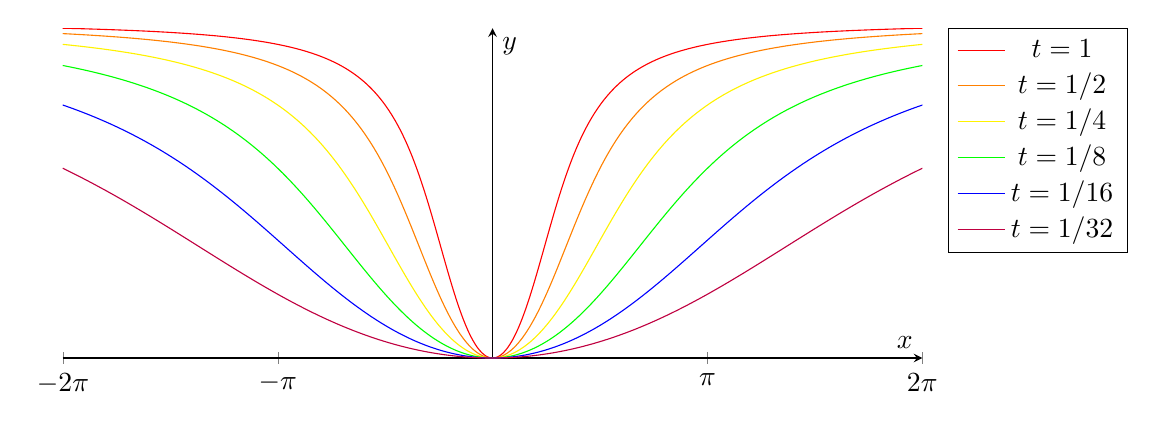
\begin{tikzpicture}
    \begin{axis}[
        xlabel=$x$,
        ylabel=$y$,
        width=12.5cm,
        height=5.77cm,
        xmin=-2*pi, xmax=2*pi,
        xtick={-6.28, -3.14, 0, 3.14, 6.28},
        xticklabels={$-2\pi$, $-\pi$, $0$, $\pi$, $2\pi$},
        ytick=\empty,
        axis lines=middle,
        samples=200,
        smooth,
        domain=-2*pi:2*pi,
        legend pos=outer north east,
    ]
    \addplot[red] {atan(x^2)};
    \addlegendentry{$t=1$}
    
    \addplot[orange] {atan(1/2*x^2)};
    \addlegendentry{$t=1/2$}
    
    \addplot[yellow] {atan(1/4*x^2)};
    \addlegendentry{$t=1/4$}
    
    \addplot[green] {atan(1/8*x^2)};
    \addlegendentry{$t=1/8$}
    
    \addplot[blue] {atan(1/16*x^2)};
    \addlegendentry{$t=1/16$}

    \addplot[purple] {atan(1/32*x^2)};
    \addlegendentry{$t=1/32$}
    \end{axis}
\end{tikzpicture}
    \end{center}
    \begin{enumerate}
        \item Montrer que \(F\) est bien définie et déterminer \(\lim_{t\to+\infty}F(t)\).
        
        \item Montrer que \(F\) est continue sur \(\R_+\).
        \item Montrer que \(F\) est dérivable sur \(\R_+^\ast\) et exprimer \(F'\)
        sous la forme d'une intégrale dépendant d'un paramètre. (Indication: montrer
        que \(F\) est dérivable sur tout intervalle de la forme \(\oo{a,+\infty}\) avec
        \(a>0\).)
        \item Donner une condition suffisante pour que la fonction \(F\) soit dérivable en \(0\).
        Que vaut alors \(F'(0)\)?
    \end{enumerate}
\end{td-exo}
% ----- Solutions exo 7
\iftoggle{showsolutions}{
    \begin{td-sol}[]\,
        \begin{enumerate}
            \item On remarque que la mesure est finie et donc les fonctions
            constantes sont intégrables. On a alors
            \begin{equation*}
                \n{\arctan(x^2t)}\leq \frac{\pi}{2}\quad \forall t\leq 0, \forall x\in\R
            \end{equation*}
            et alors
            \begin{equation*}
                \n{F(t)}\leq\int_{\R}\n{\arctan(x^2t)}\der\mu(x)\leq \frac{\pi}{2}\mu(\R)=C\in\R
            \end{equation*}
            et donc \(F\) est bien définie.

            On considère \({\left(t_n\right)}_{n\in\N}\) une suite de réels positifs qui
            converge vers \(+\infty\). On regarde alors la
            limite de \(F(t_n)\) et on utilise le théorème de convergence dominée.

            On vérifie les hypothèses en remarquant que la limite simple
            vaut \(\frac{\pi}{2}\one_{\R^\ast}(x)\).

            Pour la domination on a déjà trouvé la fonction constante \(\frac{\pi}{2}\) qui majore les \(F(t_n)\)
            et qui est intégrable.

            On peut donc appliquer le théorème de convergence dominée pour obtenir
            \begin{equation*}
                \lim_{n\to+\infty}F(t_n) = \int_{\R}\frac{\pi}{2}\der\mu(x) = \frac{\pi}{2} \mu(\R^\ast).
            \end{equation*}
            
            \item Montrons que \(F\) est continue sur \(\R_+^\ast\) et puis sur \(\R_+\).

            Pour \(t\in\R_+^\ast\) fixé, on a 
            \begin{equation*}
                \n{\arctan(x^2t)}\leq \frac{\pi}{2}\quad \forall x\in\R_+
            \end{equation*}
            à \(x\) fixé,
            \begin{equation*}
                t\mapsto \arctan(x^2t)
            \end{equation*}
            est \(C^\infty\) et donc continue.

            Pour l'argument de domination, on a la majoration et par le théorème
            de continuité sous le signe intégrale, on a \(F\) continue sur \(\R_+^\ast\).

            Enfin, pour \(t=0\), on regarde la limite à droite.
            \(\triangleright\) Le même argument de domination nous donne que
            \begin{equation*}
                \lim_{n\to+\infty}\arctan{x t_n} = \arctan(0) = 0
            \end{equation*}
            et donc
            \begin{equation*}
                F(0)=\int 0 = 0
            \end{equation*}
            et donc \(F\) est continue sur \(\R_+\).

            \item Soit \(a>0\). On prend \(t\in\oo{a,+\infty}\) et on étudie la dérivabilité de \(F\) en \(a\).

            \(\triangleright\) Si \(t\geq a\) fixé, on a
            \begin{equation*}
                x\mapsto \arctan(x^2t) \leq \frac{\pi}{2}\in\scr L^1(\mu)
            \end{equation*}

            \(\triangleright\) Si \(x\in \R\) fixé, on a
            \begin{equation*}
                t\mapsto \arctan(x^2t)
            \end{equation*}
            est dérivable sur \(\R_+^\ast\)

            \(\triangleright\) On peut donc appliquer la domination:
            \begin{equation*}
                \n{\frac{\partial}{\partial t}\arctan(x^2t)}
                = \n{x^2\frac{1}{1+x^4t^2}}\leq M\in\R
            \end{equation*}
            On voit tout de suite l'importance de \(t>a\). Si \(t=0\), on
            devrait majorer \(x^2\), ce qui est absurde.

            Or
            \begin{equation*}
                M = \sup_{x\in\R}\n{x^2\frac{1}{1+x^4a^2}}<+\infty
            \end{equation*}
            car c'est une fonction continue qui s'annule en \(+\infty\) et qui tend
            vers 0 en 0.

            On peut donc appliquer le théorème de dérivation sous le signe intégrale
            pour obtenir que \(F\) est dérivable sur \(\oo{a,+\infty}\) et que
            \begin{equation}
                F'(t) = \int_{\R}\frac{x^2}{1+x^4t^2}\der\mu(x)\label{eq:arctan_exo_7_3}
            \end{equation}

            Comme \(\eqref{eq:arctan_exo_7_3}\) est vérifiée pour tout \(t\in\oo{a,+\infty}\)
            avec \(a>0\), on en déduit que \(F\) est dérivable sur \(\R_+^\ast\).
            
            \item Si on suppose que \(\int x^2\der\mu(x)<+\infty\), alors
            \(F'(0)\) est bien définie et vaut
            \begin{equation*}
                F'(0) = \int_{\R}x^2\der\mu(x)
            \end{equation*}
        \end{enumerate}
    \end{td-sol}
}{}

\begin{td-exo}[] % 8
    A remplir
\end{td-exo}

\begin{td-exo}[] % 9
    Montrer qu'il existe une partie mesurable \(A\in\scr A\) telle que
    \(f=\one_A\) presque partout.
\end{td-exo}

\iftoggle{showsolutions}{
    \begin{td-sol}[]\,
        Rapide à faire, on fait passer f de l'autre coté, on factorise
        et on utilise que f vaut 0 ou 1 presque partout, soit par
        image reciproque, f vaut \(\one_A\) presque partout.
    \end{td-sol}
}{}

